%Layout
	\documentclass[a4paper, twocolumn, twoside, 11pt]{article}
	\setlength{\columnsep}{1cm}
	\setlength{\parskip}{6pt}
	%\usepackage{geometry}
	\usepackage[margin=1.5cm]{geometry}
	\usepackage{float}
	%\usepackage{multicol}
	\usepackage{tocloft}
	\renewcommand\cftsecafterpnum{\vskip-5pt}
	%\usepackage{hyperref}

%fonts
	\usepackage[T1]{fontenc}
	\usepackage[sfdefault]{roboto}
	\usepackage[T1]{fontenc}
	\usepackage[usenames, dvipsnames]{color}
	
%URLs
	\usepackage[colorlinks=true,
				linkcolor=black,
				urlcolor=WildStrawberry]{hyperref}
	

%Code listings
	
	\usepackage{listings}
	\definecolor{code}{rgb}{0.95,0.95,0.95}
	\definecolor{codeframe}{rgb}{0.9,0.9,0.9}
	
	\lstset{
		frame=single,
		numbers=left,
		numbersep=10pt,
		tabsize=8,
		basicstyle=\footnotesize\ttfamily,
		rulecolor=\color{codeframe},
		backgroundcolor=\color{code}
		}

	%Python Specific
	\definecolor{pcomment}{RGB}{207,0,19}
	\definecolor{pkey}{RGB}{241,117,34 }
	\definecolor{pcode}{rgb}{0.95,0.95,1.0}
	\definecolor{pcodeframe}{rgb}{0.8,0.8,1.0}
	\definecolor{codenumber}{rgb}{0.5,0.5,0.5}
	
	\lstdefinestyle{python}{
		language=Python,
		rulecolor=\color{pcodeframe},
		backgroundcolor=\color{pcode},
		keywordstyle=\color{pkey},
		commentstyle=\color{pcomment},
		numberstyle=\tiny\color{codenumber},
		emphstyle=\color{purple},
		showstringspaces=false,
		tabsize=4,
		breaklines=true
		}
	\usepackage{lstlangarm}
%Asides
	\usepackage{mdframed}
	\newenvironment{aside}
		{
		\begin{mdframed}[
			style=0,%
			leftline=false,
			rightline=false,
			innerbottommargin=2pt,
			innerleftmargin=12pt,
			innerrightmargin=0pt,
			linewidth=0.75pt,
			skipabove=6pt,
			skipbelow=6pt
			]
				\small
				\color{JungleGreen}
				\setlength{\parskip}{2pt}
				\vspace{2pt} %correct for parskip
		}
		{
		\end{mdframed}
		}

%Everything else
	\usepackage[utf8]{inputenc}
	\usepackage{graphicx}
	
%	-	-	-	-	-	-	-	-	-	-	-	-	-	-	-	-	-	-	-	-

\begin{document}

	\author{Manchester Raspberry Jam}
	\title{Workshop 10: ARM Assembly}
	\date{}

	\maketitle
	
	\setcounter{tocdepth}{1}
	\tableofcontents
	
	%	-	PART 0
	\setcounter{section}{-1}
	\section{Introduction}

		This workshop takes a very quick look into the ARM assembly language, how programming in assembly differs to more typical programming languages, and how the assembly code we write is relating to the Raspberry Pi hardware.
		
		This workshop is recommended for people with experience in a regular programming language such as Python.
		
		These booklets were created using {\fontfamily{rfdefault}\selectfont \LaTeX}, an advanced typesetting system used for several sorts of books, academic reports and letters.
		%Thanks to the Fribourg Open Source Community for their ARM language definition for Latex's listings package.
	
		\subsection*{What you'll need}
			Not much! programming in assembly requires no additional software, everything we need is bundled in with Raspbian. Here's what we'll be using:
	
			\begin{itemize}			
				\item A Text editor
				\scriptsize\newline At the Jam, we'll be using VIM, but any will do. If you'd like to try using VIM, install by typing the following command into the terminal:
				%\mbox{\color{WildStrawberry}sudo apt-get install vim vim-gnome\color{black}}
				\begin{lstlisting}
$ sudo apt-get install vim vim-gnome
				\end{lstlisting}
				\normalsize
			
				\item An Assembler
				\scriptsize\newline We'll be using the GNU portable assembler. This is pre-installed with Raspbian.
				\normalsize
			
				\item The files for this workshop from our Google Drive:
				\scriptsize\newline Go to \url{bit.ly/mcrraspjam}, then navigate to `Workshops $>$ 010: ARM Assembly'.
				\normalsize
			\end{itemize}
	
		\subsection*{Code listings \& asides}
	
			When you need to make changes to your code, they'll be presented in boxes like the following:

			\lstinputlisting[style=ARM]{code/0_helloworld.s}
	
			You might not need to copy everything, so check the line numbers to make sure you're not copying something twice.
			
			Terminal commands are listed as such, copy everything \textit{after} the dollar sign. Lines without dollar signs are example outputs, and do not need to be copied.
			
			\begin{lstlisting}
$ ./addition.s
$ echo $?
102
			\end{lstlisting}
	
			%Occasionally, something will be explained in greater detail in asides, like the one below. You can read these as you wish.
	
			%\begin{aside}
				%text after an @ symbol is a \textbf{comment} (until the end of that line).
				%We use comments to explain what each bit of code does, but they make no difference to how the program runs.
			%\end{aside}
			
		\subsection*{Further Reading}
			%If you want to continue experimenting with ARM assembly after this workshop, I highly recommend the book  \textit{``Raspberry Pi Assembly Language Raspbian'' [Third Edition]} by Bruce Smith, which parts of this workshop are based on.
			
			Parts of this workshop are based on \textit{``Raspberry Pi Assembly Language Raspbian'' [Third Edition]} by Bruce Smith.
		
		\subsection*{Questions?}
		
			We're just covering the basics of ARM assembly today. If you enjoy it, and want more ARM workshops, let me know!
	
			Send any corrections, suggestions or questions to:
			\url{jam@jackjkelly.com}\label{email}
		
 	\newpage
	\section{Quick Start}
	
		We won't be starting with ``Hello, World!'' today, as when we're programming at a low level, we're more interested in numbers than text.
		
		Printing text takes an extra step, which we'll try later. For now, let's start by moving some numbers about, to see how a very simple program works.
		
		\subsection*{1\_register.s}
		
			If you copied the workshop files to your Raspberry Pi, \textbf{open} the text file  titled \textit{`1\_register.s'}. Otherwise, copy out the program below:
		
			\lstinputlisting[style=ARM, firstline=1, lastline=2]{code/1_register.s}
			
			These two lines tell the computer to start below the line `\_start: '. This will be the start of every program we write.
			
			Below this line, we will write a basic program. \textbf{Copy} out the code below. Indentation and capitalisation will help you read your code, but aren't necessary.
			
			\lstinputlisting[style=ARM, firstline=3, firstnumber=3]{code/1_register.s}
			
			Let's run the program, then we can take a look at what we just created.
			
			\subsubsection*{Assembling your program}
			
				Navigate to your .s file from within a terminal. (use \textit{ls} and \textit{cd} commands) Once found, assemble your program by \textbf{typing} the following command
				
				\begin{lstlisting}
$ as -o 1_register.o 1_register.s
$ ld -o 1_register 1_register.o
				\end{lstlisting}
		
				This assembles and `links' the program we just wrote, and creates a binary executable. To run this, we can \textbf{type}:
				
				\begin{lstlisting}[firstnumber=3]
$ ./1_register
				\end{lstlisting}
				
				It would seem that nothing has happened. In fact, because there are no `print' statements in this program, it has completed without providing us any output. we can get our number 65 back, by \textbf{typing} in the console 
				
				\begin{lstlisting}[firstnumber=4]
$ echo $?
65
				\end{lstlisting}
				
				This is an OS short cut, which prints the last value of R0, which should be the 65 from our program. Let's now figure out what our program just did.
				
	\section{ARM assembly basics}
	
		Let's break down the first line we wrote:
		
		\lstinputlisting[style=ARM, firstline=4, lastline=4]{code/1_register.s}
		
		The operations we perform in assembly programs are all done using \textbf{instructions}. Apart from a couple of exceptions, instructions directly use one of the mathematical or logical functions of the Raspberry Pi CPU.
		
		Each instruction consists of a 3 to 5-letter \textbf{mnemonic}, as well as a number of \textbf{registers}, the fast memory locations we use in assembly programming.
		
		MOV is an instruction that is used to move values between registers. A value is moved from the second register to the first.
		
		In this case, we moved the number 65 into register 0. We could have used another register in place of 65, but in this case the \# symbol denotes that we are using a numeric value, and we call this a \textbf{literal}.
		
		\subsection*{Adding more instructions}
		
			let's add some more instructions to our program. the instruction ADD will perform an addition of two register locations. the instruction is used as follows:
		
			ADD <Output>, <Input 1>, <Input 2>
		
			Let's modify our program so that there are two registers with numbers held in them.
		
			\lstinputlisting[style=ARM, firstline=3, firstnumber=3, lastline=5]{code/2_addition.s}
		
			now that we have our two inputs, we can add our addition instruction to the code.
		
			\lstinputlisting[style=ARM, firstline=6, firstnumber=6, lastline=8]{code/2_addition.s}
		
			Assemble and link the program, as we did before, then re-run the program. When echoed, the output should read 102, the sum of our R0 and R1 values.
		
			\begin{lstlisting}
$ echo $?
102
			\end{lstlisting}
		
	\section{The Raspberry Pi Hardware.}
	
		\subsection*{Registers}
	
			It was mentioned previously that registers are fast memory locations that we perform operations on. There are only a few registers, which we need, because the computer's RAM is far too slow to keep up with the CPUs operation speed.
		
			There are 17 registers, each of which stores a numeric value. R0-R12 are available to be modified by our programs, but R13, R14, R15 are reserved for special purposes.
			
			To ensure the registers are running at fast speeds, they are contained within the CPU hardware.
	
		\subsection*{The CPU}
		
			\begin{figure}[h]
				\centering
				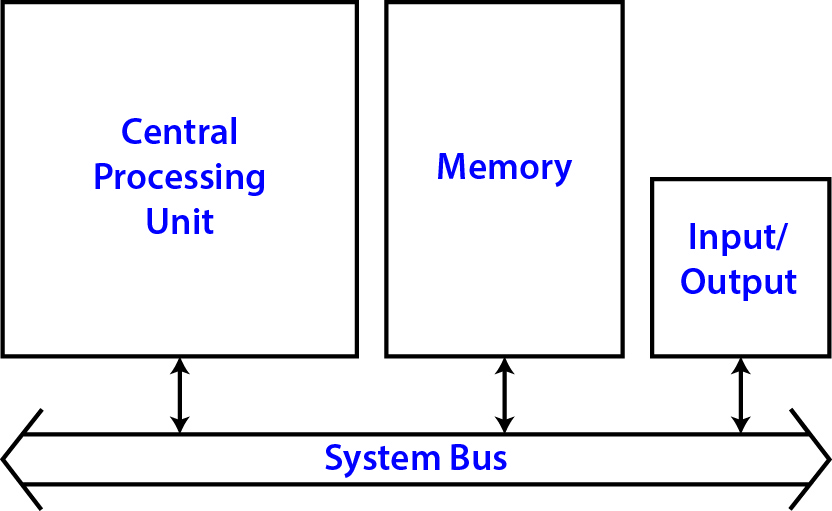
\includegraphics[width=1\linewidth]{img/3box_1}
				\caption[3 Box Model]{Single Bus Model of Computer Architecture}
				\label{fig:3box_1}
			\end{figure}
			
			Figure \ref{fig:3box_1} shows the traditional model of computer hardware. Data is moved from memory or external I/O devices into the CPU register bank, where it is operated upon, and later returned.
			
			In Assembly, we're mostly concerned with the CPU, with little attention on the memory or I/O devices. Let's fill in some detail into the CPU part of this diagram.
			
			\newpage
			There are 3 main components to a CPU:
			\begin{enumerate}
				\item The \textbf{register bank}, that holds data between CPU cycles.
				\item The hardware that performs mathematical data on our register values. We call this collected hardware the Arithmetic Logic Unit (\textbf{ALU})
				\item The \textbf{control} logic that connects these components. For each instruction, the control sends the data to different parts of the ALU, then redirects it back to the register bank.
			\end{enumerate}
			
			These components could be illustrated as shown in figure \ref{fig:3box_2} below.
			
			\begin{figure}[h]
				\centering
				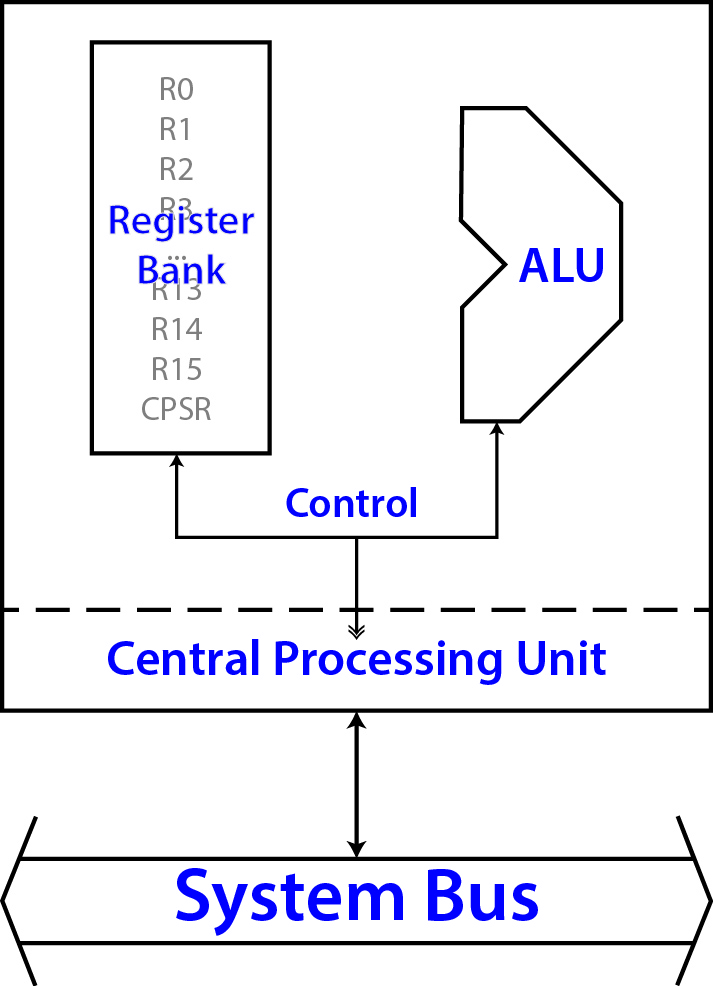
\includegraphics[width=0.7\linewidth]{img/3box_2}
				\caption[CPU box model]{The basic internal components of a CPU, at a very high level.}
				\label{fig:3box_2}
			\end{figure}
			
		\subsection*{Executing Assembly Instructions}
		
		The majority of assembly instructions are directly interpreted by the control hardware in the CPU, and each one performs a different ALU action on a number of register inputs.
		
		An assembler simply translates this instructions from textual code into their binary instruction equivalents. The assembler will also perform some more advanced functions on some non-instruction code, such as labels and psuedo instructions.
	
	\newpage
	\section{Loading from memory}
	
		Let's learn how to load data from memory. We'll need to learn how to do this in order to complete our ``Hello, World!'' program in the next section. For now, we'll just load a single number.
		
		\subsection*{3\_memory.s}
		
		We'll start with another blank file. Find and \textbf{open} \textit{3\_memory.s}
		 
		\lstinputlisting[style=ARM, firstline=1, lastline=2]{code/3_memory.s}
		
		We can store a value in memory by adding it to our assembly file, like written below.
		
		In a regular programming language, this is like a variable called `value'. `word' states that this is a 32-bit number, which is the size of each register location. \textbf{Copy} this, leaving it at the end of the file.
		
		\lstinputlisting[style=ARM, firstline=13, firstnumber=-2]{code/3_memory.s}
		
		Remember that memory is like a long list of values. Each memory location contains a value, as well as a unique address that allows that location to be found and accessed.
		
		To load from memory, we will need to first get the address. The instruction \textbf{ADR} will find the address of our memory location:
		
		\lstinputlisting[style=ARM, firstline=3, lastline=4, firstnumber=3]{code/3_memory.s}
		
		We can now load the number from memory. The \textbf{LDR} instruction loads a memory value from a given address; the square brackets around R1 show that this register contains an address, not a number.
		
		\lstinputlisting[style=ARM, firstline=5, lastline=7, firstnumber=5]{code/3_memory.s}
		
		Our number should now be in R0. We will end this program as before.
		
		\lstinputlisting[style=ARM, firstline=8, lastline=12, firstnumber=8]{code/3_memory.s}
		
		Assemble, link and run the program as before. The output from echo should be:
		
		\begin{lstlisting}
$ echo $?
72
		\end{lstlisting}

	\section{``Hello, World!''}
	
		\subsection*{printing \textit{value}}
	
			Sticking with the memory program for now, let's try outputting our loaded memory value as text in the terminal.
	
			We'll be using an instruction called `software interrupt' (\textbf{SWI}) to print text. This instruction will call to an external program within the operating system, which will print text for us.
	
			Because of the complexity of the external program, we need to give it parameters by setting the following registers
	
			\begin{figure}[h]
			\begin{tabular}{|c|l|l|}
				\hline \textbf{Register} & \textbf{Purpose} & \textbf{Value Used} \\ 
				\hline R7 & Program to Run & 4 (print) \\ 
				\hline R0 & Output Stream & 1 (terminal) \\ 
				\hline R2 & String Length & 1\\ 
				\hline R1 & String Address & value\\ 
				\hline 
			\end{tabular}
			\caption[print]{Printing parameters}
			\label{fig:print}
			\end{figure}
	
			As R0 is used by SWI, we will load our value to R1 instead of R0. We will set all of these values as such:
	
			\lstinputlisting[style=ARM, firstline=3, lastline=10, firstnumber=3]{code/4_print.s}
	
			note that we no longer need to load our value, as we only require the address for the SWI call.
	
			Try assembling, linking and running the program again. The output is a little odd, can you think why this is?
			
			\begin{lstlisting}
$ ./4_print.s
H $
			\end{lstlisting}
			
		\subsection*{Printing ``Hello, World!''}
		
		We could load each letter in turn, like our current program, but thankfully the assembler contains some useful short cuts for writing strings.
		
		Let's remove value at the end of our file, and add our hello world string instead.
		
		\lstinputlisting[style=ARM, firstline=17, firstnumber=-2]{code/5_helloworld.s}
		
		When your program is assembled, this string will be turned into a succession of ASCII numbers, just as we need them.
		
		Now we just need to change a couple of things. Make sure ADR is loading string, not value, and make sure that, as stated in figure \ref{fig:print}, the length of the string is correct. (14 for me. Spaces count, \textbackslash n is 1 ASCII character)
		
		Try assembling, linking and running the program again. With any luck, you've finally reached ``Hello, World!'' in assembly.
		
		\begin{lstlisting}
$ ./5_helloworld.s
Hello, World!
$
		\end{lstlisting}

\section{Completed Code Listings}

\textbf{1\_register.s}
\lstinputlisting[style=ARM]{code/1_register.s}

\textbf{2\_addition.s}
\lstinputlisting[style=ARM]{code/2_addition.s}

\textbf{3\_memory.s}
\lstinputlisting[style=ARM]{code/3_memory.s}

\newpage
\textbf{4\_print.s}
\lstinputlisting[style=ARM]{code/4_print.s}

\textbf{5\_helloworld.s}
\lstinputlisting[style=ARM]{code/5_helloworld.s}

\end{document}